% !TEX root = ../AnonymousSubmission2027.tex
\section{Method}

\subsection{Method Overview}

\begin{figure*}[t]
    \centering
    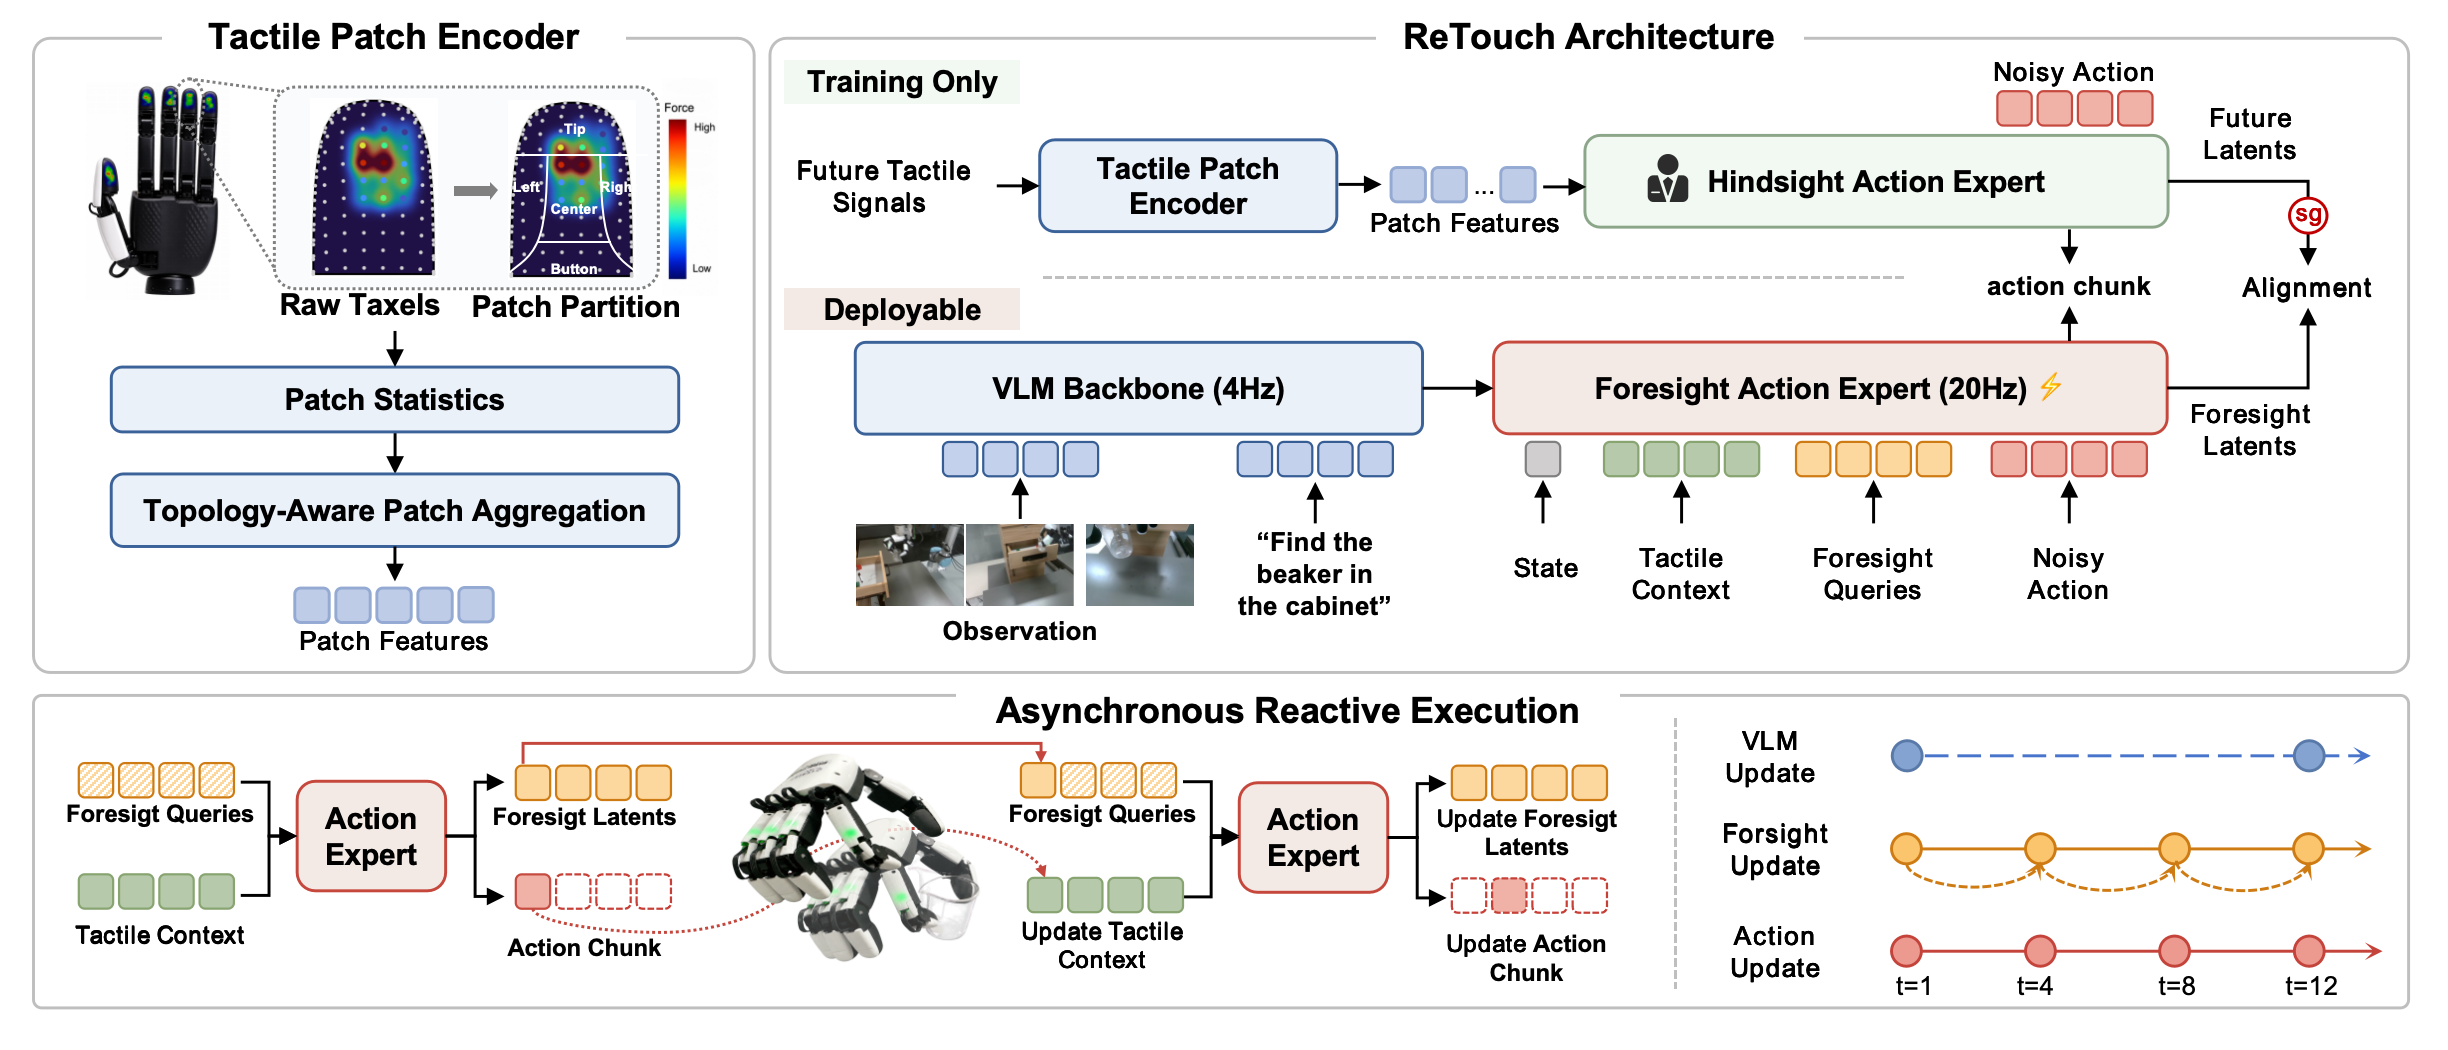
\includegraphics[width=\textwidth]{Figures/framework_draft.png}
    \caption{Overview of \systemname. The framework combines structured tactile patch encoding, action-relevant tactile foresight learning, and asynchronous closed-loop refinement of future tactile latents and action chunks.}
    \label{fig:framework}
\end{figure*}

We propose \systemname, a tactile-action world model for contact-rich dexterous manipulation that recursively refines future tactile latents and action chunks during execution. As shown in Fig.~\ref{fig:framework}, \systemname\ separates low-frequency vision-language reasoning from high-frequency joint revision of tactile foresight and actions. Specifically, we denote the semantic context cached by the VLM at the \(k\)-th low-frequency update as \(c_k\), and the chunk-start robot state as \(s_k\). At each high-frequency call \(t\), the Action Expert takes \(c_k\), \(s_k\), the observed tactile context \(\mathcal{T}_t\), and the future tactile latents from the previous call as input. Here, \(\mathcal{T}_t\) denotes the current and historical tactile observations available at time \(t\). The Action Expert updates the future tactile latents \(\hat{Z}_t^{+}\) and regenerates the action chunk \(\hat{A}_t\), allowing action generation to rely on both recent tactile feedback and a recursively refined tactile foresight representation. To make this recursive foresight operate on structured tactile inputs, \systemname\ uses a Tactile Patch Encoder to organize tactile observations across the five fingers into tactile patch features. During training, a Hindsight Action Expert extracts action-relevant future tactile targets from ground-truth future tactile patch features. A deployable Foresight Action Expert then learns to infer the corresponding future tactile latents for online foresight and action revision.

\subsection{Structured Tactile Patch Encoding}


Tactile signals from a dexterous hand are high-dimensional and sparse, yet they follow a local contact structure. For example, in XHand, each finger contains 120 three-dimensional force taxels, giving an 1800-dimensional tactile observation per frame across five fingers. Flattening all taxels into the policy would force the model to infer task-relevant contact regions from complex point-level signals. Effective contacts in dexterous manipulation, however, often occur on functional regions such as the finger tip or finger sides. We therefore design a Tactile Patch Encoder that explicitly models local contact topology within each finger and converts high-dimensional tactile readings into structured finger representations. Specifically, we divide the 120 taxels on each finger into five functional contact patches: tip, center, base, left, and right. For each patch \(p\), the encoder estimates soft contact weights from taxel force magnitudes and aggregates local tactile statistics:
\begin{equation}
    u_{t}^{i,p}
    =
    \mathrm{Agg}
    \big(\{\tau_{t}^{i,j} \mid j \in \mathcal{P}_{p}\}\big),
\end{equation}
where \(\tau_{t}^{i,j}\) denotes the force reading of taxel \(j\) on finger \(i\), \(\mathcal{P}_{p}\) denotes the taxels belonging to patch \(p\), and \(u_{t}^{i,p}\) contains weighted mean force, maximum absolute force, contact area, and contact strength. These patch-level statistics pass through a shared projection network and are combined with finger and patch embeddings, producing patch features with both finger identity and local contact identity.

To preserve local contact structure without increasing the policy-facing token count, the Tactile-Patch Encoder does not expose all patch tokens to the policy. It instead performs contact-aware pooling over the five patch features within each finger, producing one finger-level tactile token:
\begin{equation}
    z_t^{\mathrm{tac}}
    =
    E_{\phi}(\tau_t)
    =
    \{z_t^1,\ldots,z_t^{N_f}\}, \quad N_f=5 .
\end{equation}
The policy therefore receives only five tactile tokens per frame, while each token retains patch-level contact information inside the corresponding finger.

We pretrain the Tactile-Patch Encoder before policy training to obtain stable local contact representations. During pretraining, the encoder extracts finger-level patch tactile features from raw tactile readings, followed by three lightweight prediction heads for structural supervision. These heads predict the contact-strength distribution over patches, the tactile summary statistics of each patch, and whether each patch is in contact. We then load the pretrained Tactile-Patch Encoder into the policy model. During the early stage of policy training, the encoder is frozen so that the action model learns from stable tactile representations. It is later optimized end-to-end, allowing the tactile representation to adapt to the action generation objective.

\subsection{Action-Relevant Tactile Foresight Learning}

After obtaining structured tactile patch features, we learn patch-aware future tactile latents that the policy can predict. These latents are built from the tactile patch features produced by the Tactile-Patch Encoder and encode future contact information useful for action generation. The policy therefore predicts a structured future tactile representation rather than reconstructing high-dimensional, taxel-level future touch.

To obtain action-relevant future tactile representations, we train with two Action Experts. The Hindsight Action Expert produces supervision targets, and the Foresight Action Expert learns to predict future tactile latents. The Hindsight Action Expert is a privileged branch with access to ground-truth future touch. Future tactile patch features encoded from ground-truth future touch are provided as conditions to this branch. Because the Hindsight Action Expert is trained with the action generation objective, its internal future tactile token representations are shaped toward contact factors that support action prediction. We use the hidden states of future tactile tokens from its penultimate block as action-relevant future tactile targets:
\begin{equation}
    Y^{\mathrm{hid}}
    =
    \mathrm{HAE}_{L-1}
    \big(c_k, s_k, \mathcal{T}_t, E_{\phi}(\tau_{t:t+H}^{+})\big),
\end{equation}
where \(L-1\) denotes the penultimate block, and \(\tau_{t:t+H}^{+}\) denotes the ground-truth future tactile sequence available only during training.

The Foresight Action Expert follows the deployable policy conditioning and uses learnable Tactile Foresight Queries to form patch-aware future tactile latents from the available context. We take the hidden states of these foresight latents from the penultimate block of the Foresight Action Expert:
\begin{equation}
    Y^{\mathrm{fore}}
    =
    \mathrm{FAE}_{L-1}
    \big(c_k, s_k, \mathcal{T}_t, Q^{\mathrm{fore}}\big),
\end{equation}
where \(Q^{\mathrm{fore}}\) denotes the Tactile Foresight Queries. We then align \(Y^{\mathrm{fore}}\) to the action-relevant future tactile targets \(Y^{\mathrm{hid}}\):
\begin{equation}
    \mathcal{L}_{\mathrm{align}}
    =
    d\big(Y^{\mathrm{fore}}, \mathrm{sg}(Y^{\mathrm{hid}})\big),
\end{equation}
where \(d(\cdot,\cdot)\) is the latent alignment distance and \(\mathrm{sg}(\cdot)\) denotes stop-gradient. Through this latent alignment, the Foresight Action Expert learns to infer control-relevant, patch-aware future tactile latents from current and historical tactile observations. At deployment, the Hindsight Action Expert is removed, and only the Foresight Action Expert is retained.

\subsection{Asynchronous Closed-Loop Tactile Foresight}

Although the Foresight Action Expert can predict patch-aware future tactile latents, one-shot open-loop tactile foresight is not sufficient for long-horizon contact control. Predicting tactile evolution over a long action chunk can accumulate errors. Slip, contact shifts, object deformation, and execution errors can also change the interaction state, making the original tactile forecast inconsistent with the revised action plan. \systemname\ therefore turns future tactile latents from open-loop predictions into recursively updated execution states, and uses them to close the loop between tactile foresight and the unexecuted actions.

\systemname\ uses a multi-rate asynchronous execution mechanism that separates low-frequency semantic reasoning from high-frequency contact correction. The VLM receives visual observations and language instructions at 4 Hz, then produces and caches a semantic context. The Action Expert runs at 20 Hz and is invoked multiple times between consecutive VLM updates. At each high-frequency call, the Action Expert reuses the cached VLM context and chunk-start robot state, while incorporating the current observed tactile context and the future tactile latents from the previous call. The recursive update is written as
\begin{equation}
    (\hat{Z}_{t}^{+}, \hat{A}_{t})
    =
    \mathrm{FAE}_{\theta}
    \big(c_k, s_k, \mathcal{T}_t, \hat{Z}_{t^-}^{+}\big),
\end{equation}
where \(\hat{Z}_{t}^{+}\) denotes the updated future tactile latents, \(\hat{A}_{t}\) denotes the regenerated action chunk, and \(\hat{Z}_{t^-}^{+}\) denotes the future tactile latents from the previous high-frequency call. After a short segment of actions is executed, the new tactile feedback is added to the observed tactile context and triggers the next high-frequency call. This loop lets the model adjust tactile foresight and action plans to changing tactile feedback without repeatedly running the VLM.

To ensure that each action revision is conditioned on the tactile foresight updated in the current call, we use an attention mask in the Foresight Action Expert. Tactile Foresight Queries can attend to the semantic context, robot state, observed tactile context, and the future tactile latents from the previous call, but not to action tokens. In contrast, action tokens can attend to the updated future tactile latents. This mask imposes a directional information flow: the model first forms the current future tactile latents, and then generates the action chunk conditioned on these updated latents. It prevents action-token information from leaking into future tactile latents and makes action generation depend on the latest tactile foresight.

Training and deployment use the same recursive revision form. During training, we randomly sample an offset within an action chunk and construct the corresponding observed tactile context, future tactile latent prefix, and supervision for the unexecuted actions. The model learns to continue revising future tactile latents and action chunks from intermediate execution states. During deployment, the Action Expert is invoked repeatedly at the high-frequency control rate. Each invocation regenerates an action chunk, but only the actions after the current time are executed. This design aligns random-offset revision during training with online closed-loop revision during deployment.

\subsection{Training Objectives}

\systemname\ is trained with a patch-encoder pretraining objective and a policy objective. For Tactile-Patch Encoder pretraining, we attach three lightweight prediction heads after the encoder to supervise the patch contact-strength distribution, patch tactile summary statistics, and patch contact mask. The pretraining objective is
\begin{equation}
    \mathcal{L}_{\mathrm{pre}}
    =
    \lambda_{\mathrm{dist}}\mathcal{L}_{\mathrm{dist}}
    +
    \lambda_{\mathrm{sum}}\mathcal{L}_{\mathrm{sum}}
    +
    \lambda_{\mathrm{contact}}\mathcal{L}_{\mathrm{contact}},
\end{equation}
where the three terms correspond to patch contact-strength distribution, patch tactile summary statistics, and patch contact prediction, respectively. This encourages each finger-level tactile token to retain local patch-level contact structure. After pretraining, the prediction heads are discarded, and only the Tactile-Patch Encoder parameters are kept.

For policy training, we optimize an action generation loss and the future tactile latent alignment loss defined above. The action loss is applied to both the Hindsight Action Expert and the Foresight Action Expert, so both branches learn to generate action chunks. The Hindsight targets are treated as stop-gradient targets during alignment, so the alignment loss updates only the Foresight Action Expert and does not alter the target representations from the Hindsight branch. The final policy objective is
\begin{equation}
    \mathcal{L}_{\mathrm{policy}}
    =
    \mathcal{L}_{\mathrm{act}}^{\mathrm{hid}}
    +
    \mathcal{L}_{\mathrm{act}}^{\mathrm{fore}}
    +
    \lambda_{\mathrm{align}}\mathcal{L}_{\mathrm{align}}.
\end{equation}